% Homework template for Inference and Information
% UPDATE: September 26, 2017 by Xiangxiang
\documentclass[a4paper]{article}
\usepackage{ctex}
\ctexset{
	proofname = \heiti{Proof}
}
\usepackage{amsmath, amssymb, amsthm}
% amsmath: equation*, amssymb: mathbb, amsthm: proof
\usepackage{moreenum}
\usepackage{mathtools}
\usepackage{url}
\usepackage{bm}
\usepackage{enumitem}
\usepackage{graphicx}
\usepackage{subcaption}
\usepackage{booktabs} % toprule
\usepackage[mathcal]{eucal}
\usepackage[thehwcnt = 4]{iidef}
\usepackage{ragged2e}
\usepackage{microtype}

\thecourseinstitute{SUSTech}
\thecoursename{Machine-learning}
\theterm{Fall 2020}
\hwname{Homework}
\slname{\heiti{Solution}}
\justifying\let\raggedright\justifying
\begin{document}
	\courseheader
	\name{Liu Yuxi}
	\begin{enumerate}
		\setlength{\itemsep}{3\parskip}
		\item
		Show that maximization of the class separation criterion given by $m_2 - m_1 = w^T(m_2- m_1) $ with respect ot $w$, using a Lagrange multiplier to enforce the constraint $w^Tw = 1$, leads to the result that $w \propto (m_2 - m_1)$.
		\begin{solution}
			We construct the Lagrangian function
			\begin{equation*}
				L=w^T(m_2-m_1)+\lambda(w^Tw-1)
			\end{equation*}
			Taking the gradient of $L$ we obtain
			\begin{equation*}
				\delta L=m_2-m_1+2\lambda w
			\end{equation*}
			setting this gradient to zeros
			\begin{equation*}
				w=-\frac{1}{2\lambda}(m_2-m_1)
			\end{equation*}
			and we get
			\begin{equation*}
				w \propto (m_2-m_1)
			\end{equation*}
		\end{solution}
		\item
		Show that the Fisher criterion
		\begin{equation*}
			\begin{aligned}
				j(w) = \frac{(m_2 - m_1)^2}{s_1^2 + s_2^2}
			\end{aligned}
		\end{equation*}
		can be written in the form
		\begin{equation*}
			j(w) = \frac{w^TS_Bw}{w^TS_Ww}
		\end{equation*}
		\begin{solution}
			\begin{equation*}
				\begin{aligned}
				(m_2-m_1)^2 &=(w^T(m_2-m_1))^2\\
				&=w^T(m_2-m_1)(m_2-m_1)^Tw\\
				&=w^TS_Bw
				\end{aligned}
			\end{equation*}
			\begin{equation*}
				\begin{aligned}
				s_1^2 + s_2 ^2&= \sum_{n \in C_1}(y_n - m_1)^2 + \sum_{k \in C_2}(y_k - m_2)^2\\
				&=\sum_{n \in C_1}(w^T(x_n - m_1))^2 + \sum_{k \in C_2}(w^T(x_k - m_2))^2\\
				&=\sum_{n \in C_1}w^T(x_n - m_1)(x_n - m_1)^Tw+\sum_{k \in C_2}w^T(x_k - m_2)(x_k - m_2)^Tw\\
				&=w^TS_Ww
				\end{aligned}
			\end{equation*}
			Finally, we obtain
			\begin{equation*}
				j(w) = \frac{w^TS_Bw}{w^TS_Ww}
			\end{equation*}
		\end{solution}
		
		\item
		Consider a agenerative classification model for K classes defined by prior class probabilities $p(C_k)=\pi_k$ and general class-conditional dendities $p(\phi | C_k)$ where $\phi$ is the input feature vector. Suppose we are given a training data set$\{\phi_n,t_n\}$ where $n=1,...,N,$ and $t_n$ is a binary target vector of length K that uses the 1-of-K coding scheme, so that it has components $t_{nj} = I_{jk}$ if pattern n is from class $C_k$. Assuming that data points are drown independently from this model, show that the maximum-likelihood solution for the prior probabilities is given by
		\begin{equation*}
			\pi_k = \frac{N_k}{N}
		\end{equation*}
		where $N_k$ is the number of data points assigned to class $C_k$.
		\begin{solution}
			The likelihood is 
			\begin{equation*}
				p(\{\phi_n,t_n\}|{\pi_k})=\prod_{n=1}^{N}\prod_{k=1}^{K}\{p(\phi_n|C_k)\pi_k\}^{t_{nk}}
			\end{equation*}
			taking the logarithm
			\begin{equation*}
				\ln p(\{\phi_n,t_n\}|{\pi_k})=\sum_{n=1}^{N}\sum_{k=1}^{K}t_{nk}\{\ln p(\phi_n|C_k)+\ln \pi_k\}
			\end{equation*}
			with the constraint $\sum_k \pi_k=1$, and we use Lagrange
			\begin{equation*}
				\ln p(\{\phi_n,t_n\}|\{\pi_k\})+\lambda(\sum_{k=1}^{K}\pi_k-1)
			\end{equation*}
			\begin{equation*}
				\sum_{n=1}^{N}\frac{t_{nk}}{\pi_k} + \lambda = 0
			\end{equation*}
			\begin{equation*}
				-\pi_k\lambda = \sum_{n=1}^{N}t_{nk}=N_k
			\end{equation*}
		\end{solution}
		\item 
		Verify the relation
		\begin{equation*}
			\frac{d\sigma}{da}=\sigma(1-\sigma)
		\end{equation*}
		for the derivative of the logistic sigmoid function defined by
		\begin{equation*}
			\sigma(a) = \frac{1}{1+\exp(-a)}
		\end{equation*}
		\begin{solution}
			\begin{equation*}
			\begin{aligned}
				\frac{da}{d\sigma}&=\frac{1}{\frac{d\sigma}{da}}\\
				&=\frac{1}{\sigma(1-\sigma)}\\
				&=\frac{1}{\sigma}+\frac{1}{1-\sigma}\\
				a(\sigma)&=\ln \sigma - \ln (1-\sigma)\\
				&=\ln \frac{\sigma}{1-\sigma}\\
				e^a&=\frac{\sigma}{1-\sigma}\\
				\sigma&=\frac{e^a}{1+e^a}\\
				&=\frac{1}{1+\exp (-a)}
			\end{aligned}
			\end{equation*}
		\end{solution}
		\item
		By making use of the result
		\begin{equation*}
			\frac{d\sigma}{da}=\sigma(1-\sigma)
		\end{equation*}
		for the derivative of the logistic sigmoid, show that the derivative of the error function for the logistic regression model is given by
		\begin{equation*}
			\bigtriangledown \mathbb{E}(w)=\sum_{n=1}^{N}(y_n-t_n)\phi_n
		\end{equation*}
		\begin{solution}
			\begin{equation*}
				\begin{aligned}
				\frac{\partial E}{\partial y_n} &= \frac{1-t_n}{1-y_n} - \frac{t_n}{y_n}\\
				&=\frac{y_n(1-t_n) - t_n (1-y_n)}{(1-y_n)y_n}\\
				&=\frac{y_n - y_nt_n - t_n + y_nt_n}{(1-y_n)y_n}\\
				&=\frac{y_n - t_n}{y_n(1-y_n)}
				\end{aligned}
			\end{equation*}
			and use
			\begin{equation*}
			\frac{d\sigma}{da}=\sigma(1-\sigma)
			\end{equation*}
			we get
			\begin{equation*}
				\frac{\partial y_n}{\partial a_n} = \frac{\partial \sigma(a_n)}{\partial a_n} = y_n(1-y_n)				
			\end{equation*}
			\begin{equation*}
				\nabla a_n = \phi_n
			\end{equation*}
			Using the chain rule, we obtain
			\begin{equation*}
			\begin{aligned}
				\nabla E &= \sum_{n = 1}^{N} \frac{\partial E}{\partial y_n}\frac{\partial y_n}{\partial a_n}\nabla a_n\\
				&= \sum_{n = 1}^{N}(y_n - t_n) \phi_n
			\end{aligned}
			\end{equation*}
		\end{solution}
		\item
		There are several possible ways in which to generalize the concept of linear discriminant functions from two classes to c classes. One possibility would be to use $(c-1)$ linear discriminant functions, such that $y_k(x)>0$ for inputs x in class $C_k$ and $y_k(x) < 0$ for not in class $C_k$. By drawing a simple example in two dimensions for $c=3$, show that this approach can lead to regions of x-space for which the classification is ambiguous. Another approach would be to use one discriminant functino $y_{jk}(x)$ for each possible pair of classes $C_j$ and $C_k$, such that $y_{jk}(x) >0$ for patterns in class $C_j$ and $y_{jk}(x) <0$ for patterns in class $C_k$. For c classes, we would need $c(c-1)/2$ discriminant functions. Again, by drawing a specific example in two dimensions for $c=3$, show that this approach can also lead to ambiguous regions.
		\begin{solution}
			
			\begin{figure}[htbp]
				\centering
				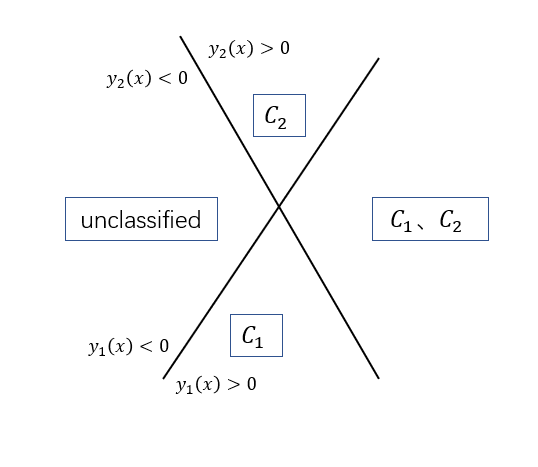
\includegraphics[width = 0.4\textwidth]{pic1.png}
				\caption{approach1 with c-1 linear discriminant functions}
				\label{fig:1}
			\end{figure}
			\begin{figure}[htbp]
				\centering
				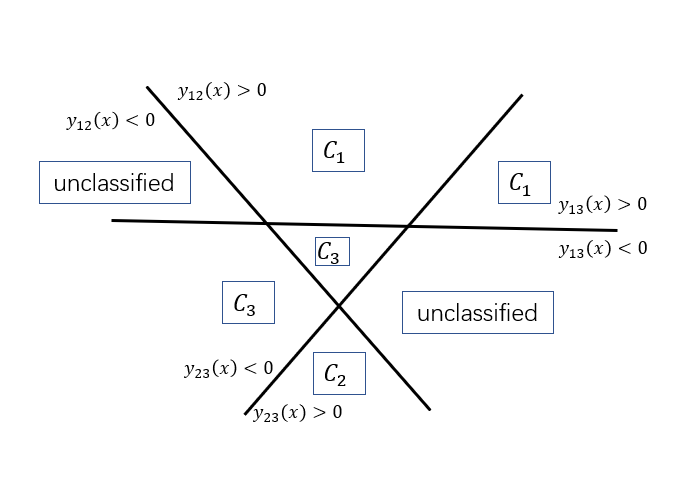
\includegraphics[width=0.4\linewidth]{pic2.png}
				\caption{approach2 with three linear discriminant}
			\end{figure}
		As for the approach1, we have two linear discriminant function. and $y_k(x)>0$ for inputs x in class $C_k$ and $y_k(x) < 0$ for not in class $C_k$. But there is still several problem, when $y_1(x)>0$ and $y_2(x)>0$, we can't judge the point belong to $C_1$ or $ C_2 $.
		
		As for the approach2, we have the classification as follows:
		\begin{enumerate}
			\item
			If $ y_{12}(x) > 0 $ and $ y_{13}(x) > 0 $, then x $\in$ $ C_1 $
			\item
			If $ y_{12}(x) < 0 $ and $ y_{23}(x) > 0 $, then x $\in$ $ C_2 $
			\item
			If $ y_{13}(x) < 0 $ and $ y_{23}(x) < 0 $, then x $\in$ $ C_3 $
		\end{enumerate}
		The follow regions are still unclassified.
		\begin{enumerate}
			\item
			$y_{12}(x) < 0$ and $y_{13}(x) > 0$.
			$y_{12}(x) > 0$ and $y_{23}(x) > 0$ and $y_{13} < 0$
		\end{enumerate}
		\end{solution}
		\item
		Given a set of data points $\{x^n\}$ we can define the convex hull to be the set of points x given by
		\begin{equation*}
			x = \sum_n \alpha_n x^n
		\end{equation*}
		where $\alpha_n >=0$ and $\sum_n \alpha_n = 1$. Consider a second set of point $\{z^m\}$and its corresponding convex hull. The two sets of points will be linearly separable if there exists a vector $\hat{w}$ and a scalar $\omega_0$ such that $\hat{w}^Tx^n+\omega_0 >0$ for all $x^n$, and $\hat{w}^Tz^m + \omega_0<0$ for all $z^m$. Show that, if their convex hulls intersect, the two sets of points cannot be linearly separable, and conversely that, if they are linearly separable, their convex hulls do not intersect.
		\begin{solution}
			we have
			\begin{equation*}
				y(x) = \hat{w}^Tx^n + w_0
			\end{equation*}
			\begin{equation*}
				x = \sum_{n} \alpha_nx^n
			\end{equation*}
			then we get
			\begin{equation*}
				y(x) = \hat{w}^T(\sum_{n}\alpha_nx_n)+w_0
			\end{equation*}
			with $ \sum_{n}\alpha_n = 1 $
			\begin{equation*}
				y(x) = \sum_{n}\alpha(\hat{w}^Tx^n+w_0)
			\end{equation*}
			Similarly we get
			\begin{equation*}
				y(z) = \sum_{m} \beta_m(\hat{w}^Tz^m + w_0)
			\end{equation*}
			If the convex hulls intersect, there must be at least one point exist in {x} and {z}. We denote this point as xz. And we get
			\begin{equation*}
				y(xz) = \sum_{n}\alpha_n(\hat{w}^T\ xz^n + w_0) = \sum_{m}\beta_m(\hat{w}^T\ xz^m + w_0)
			\end{equation*}
			But for linear separability, we have
			\begin{equation*}
				\begin{aligned}
				y(x^n) &= \hat{w}^Tx^n + w_0 > 0\\
				y(z^m) &= \hat{w}^Tz^m + w_0 > 0
				\end{aligned}
			\end{equation*}
			There is no possible for the above formulations establish simultaneously.
		\end{solution}
	\end{enumerate}
\end{document}
\begin{equation}
\end{equation}

%%% Local Variables:
%%% mode: late\rvx
%%% TeX-master: t
%%% End:
